\documentclass[aps,prl,twocolumn, superscriptaddress]{revtex4}
\usepackage[dvips]{graphicx}
\usepackage{amssymb}
\usepackage{amsmath}
\usepackage{color}



\begin{document}


\title{Insertion loss computations at subwavelength grating waveguide crossings}


\author{Daniel Hutama}
    \affiliation{Department of Physics, McGill University, Montr\'eal, Qu\'ebec, H3A 2T8, Canada}

% \author{Lawrence R. Chen}
% \affiliation{Dept. of Electrical \& Computer Engineering, McGill University, Montr\'eal, Qu\'ebec, H3A 0E9, Canada}


\date{April 17, 2019}
\begin{abstract}
\noindent \textbf{Abstract}: We report on experimental and simulation results pertaining to the insertion loss of cascaded subwavelength grating (SWG) waveguide crossings. Using three-dimensional finite-difference time-domain simulations, we compare loss characteristics of crossings proposed by Bock \textit{et. al.} with conventional strip waveguide crossings.  In addition, we show that SWG waveguides outperform strip waveguides for applications requiring multiple perpendicular planar crossings, such as in densely integrated silicon photonic structures. Although our experimental measurements fail to reproduce previous results, they highlight important considerations for the design of SWG waveguide devices.
\end{abstract}
\pacs{}
\maketitle

\section{I. Introduction}
\vspace{-1em}
Developments in silicon-on-insulator (SOI) devices show promise for new applications in several areas, such as sensing, spectroscopy, and photonic computing. Planar lightwave circuits built on these SOI platforms might require several perpendicular waveguide crossings. However, such crossings introduce significant losses to the device if implemented with conventional strip waveguides. Fortunately, subwavelength grating (SWG) waveguides make planar waveguide crossings implementable with very low loss and crosstalk \cite{BockPaper}. Our investigation aims to reproduce results presented in \cite{BockPaper} to evaluate the feasibility of using SWG waveguide meshes as a potential platform for implementing programmable photonic processors on densely integrated silicon photonic devices. 

Conventional planar strip waveguides confine light in a core of high refractive index, which is surrounded by a cladding material with low refractive index. For instance, a conventional strip waveguide might consist of a silicon (Si) waveguide core surrounded by a silica (SiO$_2$) cladding. In contrast, SWG waveguides consist of an alternating arrangement of high-refractive index and low-refractive index segments \cite{OGswg}. Figure \ref{fig:SWGdiagram} illustrates an SWG waveguide in SOI formed by a periodic arrangement of high-refractive index Si embedded within a medium of low-refractive index SiO$_2$. The SWG is characterized by a grating period $\Lambda$ and duty cycle $D= a/\Lambda$, where $a$ is the length of the high-refractive index material, measured in the direction of propagation. In addition, individual Si segments are described by a height $h$ and width $w$. 

\begin{figure}[!h]
    \centering
    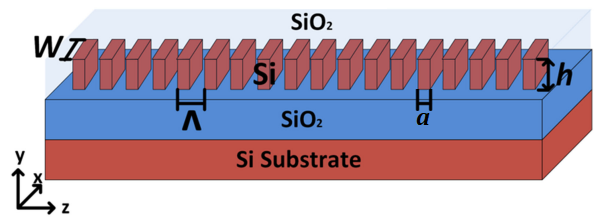
\includegraphics[width=7cm]{SWGwaveguide.png}
    \caption{Adapted from \cite{ChenPaper}. Schematic of an SWG waveguide in SOI with constant pitch $\Lambda$ and duty cycle $D = a/\Lambda$. }
    \label{fig:SWGdiagram}
\end{figure}

In conventional rectangular strip waveguides, electromagnetic fields propagate in well-understood TE/TM modes. However, electromagnetic fields in periodic grating waveguides excite Bloch-Floquet modes \cite{PhotonicCrystalsText}. These Bloch-Floquet modes are the natural modes of periodic media, and have mechanics that can be treated analogously to electron wavefunctions in a periodic crystal structure. In particular, the electric field of 
a Bloch-Floquet mode propagating through a uniform period waveguide in the $\hat{z}$ direction can be described by $E(x,y,z+\Lambda) = E_B(x,y,z)e^{-\gamma_B\Lambda}$, where $E_B(x,y,z)$ is the Bloch mode field distribution within a single period $\Lambda$, and $\gamma_B$ is the associated complex propagation constant. In general, $\gamma_B = \alpha_B + jk_B$, and $k_B = (2\pi/\lambda)n_B$, where $\alpha_B$ is the attenuation constant, $k_B$ is the propagation constant, and $n_B$ is the effective index of the Bloch-Floquet mode \cite{HalirReview}. 

For a given grating pitch $\Lambda$, the behavior of a periodic waveguide depends strongly on the free-space wavelength $\lambda$. In particular, depending on $\overline{\lambda} = \lambda/\Lambda$ (i.e. the ratio of free-space wavelength to grating pitch), the waveguide can operate in one of three regimes: (i) diffraction, in which the waveguide segments scatter an incoming beam away from the waveguide; (ii) reflection, in which an input beam from a conventional strip waveguide is reflected back into the input and gradually attenuated in the periodic waveguide; (iii) subwavelength, in which diffraction and reflection effects are suppressed \cite{HalirReview}. 

 \begin{figure}[!h]
    \centering
    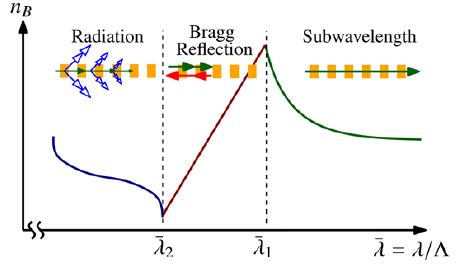
\includegraphics[width=7cm]{swgoperation.png}
    \caption{From \cite{HalirReview}. Bloch-Floquet mode effective index ($n_B$) as a function of the wavelength-to-pitch ratio $\overline{\lambda} = \lambda/\Lambda$.}
    \label{fig:SWGoperation}
\end{figure}

As shown in figure \ref{fig:SWGoperation}, light is radiated away from the waveguide for wavelengths comparable to the pitch of the grating (i.e. $\lambda/\Lambda <\overline{\lambda}_1$). Within the bandgap ($\overline{\lambda}_1<\overline{\lambda}<\overline{\lambda}_2$), the effective index follows the linear relation $n_B^{\text{Bragg}} \sim \frac{1}{2}\overline{\lambda}$. The subwavelength operating regime is reached when $n_B$ drops below the Bragg condition such that $n_B<n_B^{\text{Bragg}}$ \cite{HalirReview}. In this regime, diffraction and reflection effects are suppressed, and the SWG structure admits light as if it were a homogeneous waveguide.

One major challenge in implementing SWG waveguides lies in the transition from an input conventional strip waveguide to a periodic grating that operates in the subwavelength regime. In particular, the challenge is to design a transition that minimizes radiative and reflective effects due to differences in pitch and effective index between the two types of waveguides. In addition, the propagation modes of strip waveguides and SWG waveguides are markedly different. Thus, a direct connection between a conventional strip waveguide segment and SWG waveguide segment would result in significant losses at the interface due to mode mismatch. To curtail losses due to these effects, various interfacing structures have been proposed \cite{BockPaper}, \cite{DonzellaPaper}. Such structures generally attempt to create adiabatic transitions between propagation modes, as well as gradually change the effective index.

\vspace{-1em}
\section{II. Simulation}
\vspace{-1em}
In order to minimize insertion loss from a strip waveguide input, we first identify an effective interfacing design in a system with one crossing. After identifying an effective design, we investigate the effect of adding a second perpendicular crossing to the structure. As a starting point, we perform three-dimensional finite-difference time-domain (3D FDTD) simulations on SWG waveguide crossings detailed in \cite{BockPaper}, as well as on a conventional strip waveguide crossing. 

\vspace{-1em}
\subsection{Simulation Design and Parameters}

The design of the simulated structures is shown in figure \ref{fig:Bock}. The SWG waveguide crossing of figure \ref{fig:Bock} (top) contains a transition region between the input strip waveguide and the uniform duty cycle SWG waveguide segments near the intersection. In the transition region, the pitch $\Lambda$ is linearly chirped from $\Lambda_i = 200$ nm to $\Lambda_f = 300$ nm, and the width $w$ of each segment is gradually tapered from $w_i = 450$ nm to $w_f = 300$ nm to allow mode transitions to occur more smoothly. The length of each segment is fixed at $a=150$ nm. The transition region of figure \ref{fig:Bock} (bottom) includes constant-length bridges, which connect segments whose lengths are chirped from $a_i = 100$ nm to $a_f = 150$ nm throughout the bridged region. The segment at the intersection in both designs is a square with an area equal to that of its neighboring segments. In what follows, we refer to figure \ref{fig:Bock} (top) as the ``chirped taper'' design, and figure \ref{fig:Bock} (bottom) as the ``bridged taper'' design. 
 \begin{figure}[!h]
    \centering
    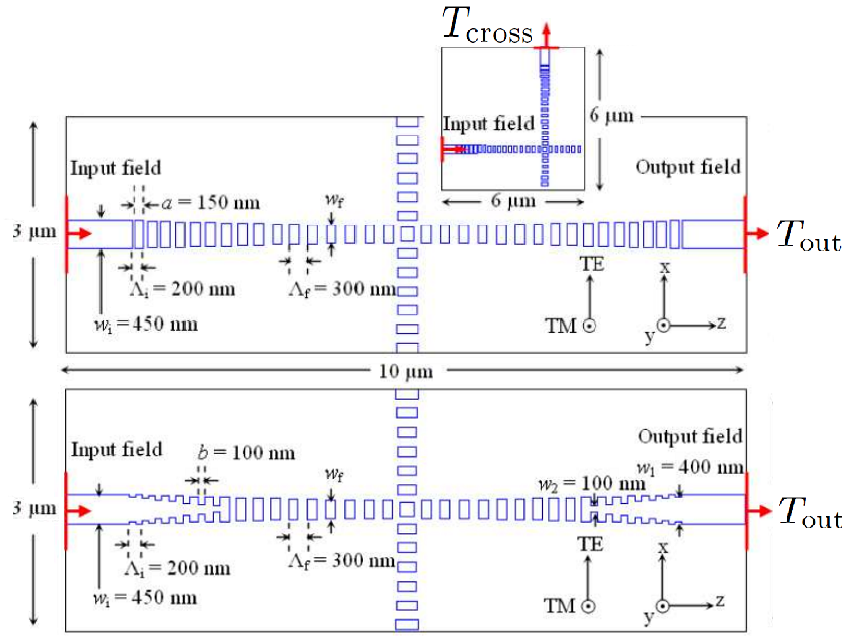
\includegraphics[width=7.8cm]{bock_cross.png}
    \caption{From \cite{BockPaper}. Schematic of SWG waveguide crossings implementing a transitional region between the input conventional strip waveguide and SWG region to reduce mode-mismatch losses.}
    \label{fig:Bock}
\end{figure}

In departure from the simulations performed by Bock \textit{et. al.} in \cite{BockPaper}, we perform our simulations over a square $xz$ region, rather than a rectangular one. Results for a square simulation region might be more relevant for future work on square waveguide meshes. In particular, we simulate over a layout region of $x\times y\times z = 10 \times 3 \times 10 \text{ }\mu\text{m}^3$, whereas Bock \textit{et. al.} simulate over a layout region with $x\times y\times z = 3 \times 3 \times 10 \text{ }\mu\text{m}^3$. The 3D FDTD simulation (Lumerical) is implemented using a non-uniform mesh, which is configured to reduce the effects of numerical dispersion at Si-SiO$_2$ interfaces. Although the mesh is non-uniform, each mesh cell satisfies a global time step of $\Delta t= 0.03845$ fs in accordance with the Courant condition: $c\Delta t\left(\frac{1}{\Delta x^{2}} + \frac{1}{\Delta y^2} + \frac{1}{\Delta z^2}\right)^{1/2} \leq 1$, where $c$ is the speed of light in vacuum. Material refractive indices used for the simulations are $n_{\text{Si}} = 3.476$, and $n_{\text{SiO}_2} = 1.444$. All simulations are performed using a source wavelength of $\lambda = 1550$ nm.

To extract useful quantitative values from our 3D FDTD simulations, we define a normalized power transmission coefficient $T = \dfrac{\frac{1}{2}\int_\mathcal{S}\text{real}(\overrightarrow{P})\cdot d\overrightarrow{A}}{\text{source power}}$, where $\mathcal{S}$ is the surface of a planar power monitor, $\overrightarrow{P}$ is the Poynting vector normal to $\mathcal{S}$, and $d\overrightarrow{A}$ is the surface normal element. With this definition, values of $T$ directly translate to the fraction of input optical power that passes through a power monitor. The size of this power monitor changes the measured $T$ value, as different sizes will capture different amounts of leakage from scattering. Thus, we perform the simulations with several sizes centered around four times the dimensions of the input waveguide. 

In our simulations, we construct power monitors to capture two $T$ values of interest indicated in figure \ref{fig:Bock}: (i) $T_{\text{out}}$, the transmission through the system, measured at the end of the arm directly opposite the source; (ii) $T_{\text{cross}}$, the crosstalk, measured at the top of the upper arm. An ideal crossing would have $T_{\text{out}}=1$ and $T_{\text{cross}} = 0$. However, we expect non-ideal values due to scattering and reflection effects in the taper regions. 

\vspace{-1em}
\subsection{Simulation Results}

As shown in table \ref{table:3dfdtd}, 3D FDTD simulations predict that both SWG waveguide crossings admit smaller values of $T_{\text{cross}}$ and higher values of $T_\text{out}$ than the conventional strip waveguide crossing. In addition, the simulation supports a result of Bock \textit{et. al.} in regards to the bridged taper design slightly outperforming the chirped taper design in both output and crosstalk dimensions \cite{BockPaper}. Comparing the bridged taper design against the conventional strip crossing, we note a thirtyfold reduction in crosstalk and significant improvement in output power.
\begin{table}[!h]
\begin{tabular}{ccccc}
\hline
\multicolumn{5}{c}{3D FDTD Simulation Output and Crosstalk Results} \\ \hline \hline
\multicolumn{1}{c|}{} & \multicolumn{1}{c|}{\begin{tabular}[c]{@{}c@{}}$T_\text{out}$\end{tabular}} & \multicolumn{1}{c|}{\begin{tabular}[c]{@{}c@{}}$T_\text{cross}$\end{tabular}} & \multicolumn{1}{c|}{\begin{tabular}[c]{@{}c@{}}Output\\ (dB)\end{tabular}} & \begin{tabular}[c]{@{}c@{}}Crosstalk\\ (dB)\end{tabular} \\ \hline
\multicolumn{1}{c|}{\begin{tabular}[c]{@{}c@{}}Conventional\\ Strip Crossing\end{tabular}} & \multicolumn{1}{c|}{$0.65(2)$} & \multicolumn{1}{c|}{$0.045(1)$} & \multicolumn{1}{c|}{$-1.87(1)$} & $-13.4(1)$ \\ \hline
\multicolumn{1}{c|}{\begin{tabular}[c]{@{}c@{}}Chirped Taper\\ SWG Crossing\end{tabular}} & \multicolumn{1}{c|}{$0.70(1)$} & \multicolumn{1}{c|}{$0.0023(4) $} & \multicolumn{1}{c|}{$-1.55(6)$} & $-26.4(8)$ \\ \hline
\multicolumn{1}{c|}{\begin{tabular}[c]{@{}c@{}}Bridged Taper\\ SWG Crossing\end{tabular}} & \multicolumn{1}{c|}{$0.72(3)$} & \multicolumn{1}{c|}{$0.0015(3)$} & \multicolumn{1}{c|}{$-1.42(2)$} & $-28.5(9)$ \\ \hline
\end{tabular}
\caption{Numerically computed transmission coefficients and corresponding decibel values for each crossing. Uncertainties were obtained by slightly varying the area of power monitors and repeating the 3D FDTD simulation.}
\label{table:3dfdtd}
\end{table}

We next wish to consider the behavior of an optical system with multiple waveguide crossings, such as a two dimensional waveguide mesh. We perform 3D FDTD simulations on a double conventional strip waveguide crossing (appendix figure \ref{fig:diagsDouble}, left), as well as on a double SWG waveguide crossing (appendix figure \ref{fig:diagsDouble}, right).
The double SWG waveguide crossing was implemented with the bridged taper design in accordance with the results of table \ref{table:3dfdtd}. The simulations are performed over a layout region of $x \times y \times z = 10 \times 3 \times 14.75 \text{ }\mu\text{m}^3$. We have increased the $z$ dimension to include a uniform strip/SWG segment between the intersecting waveguides. Larger numbers of crossing are unfeasible in terms of simulation time.

As shown in table \ref{table:3dfdtd_double}, the conventional strip waveguide double crossing has a non-negligible crosstalk coefficient. In addition, the output power suffers a significant decrease of $1.07$ dB.  On the other hand, the SWG waveguide crossing exhibits a crosstalk of less than 1\% to each arm, and a much smaller output power loss of $0.13$ dB. These simulation results suggest that SWG waveguides are superior to conventional strip waveguides for implementing circuits with many waveguide crossings. 

\begin{table}[!h]
\begin{tabular}{ccccc}
\hline
\multicolumn{5}{c}{3D FDTD Double Crossing Simulation Results} \\ \hline \hline
\multicolumn{1}{c|}{} & \multicolumn{1}{c|}{$T_{out}$} & \multicolumn{1}{c|}{$T_{\text{cross}_1}$} & \multicolumn{1}{c|}{$T_{\text{cross}_2}$} & \begin{tabular}[c]{@{}c@{}}Output\\ (dB)\end{tabular} \\ \hline
\multicolumn{1}{c|}{\begin{tabular}[c]{@{}c@{}}Conventional Strip\\ Double Crossing\end{tabular}} &  \multicolumn{1}{c|}{$0.51(2)$} & \multicolumn{1}{c|}{$0.0442(3)$} & \multicolumn{1}{c|}{$0.0372(7)$} & $-2.94(1)$ \\ \hline
\multicolumn{1}{c|}{\begin{tabular}[c]{@{}c@{}}Bridged Taper \\ Double Crossing\end{tabular}} & \multicolumn{1}{c|}{$0.70(2)$} & \multicolumn{1}{c|}{$0.0021(2)$} & \multicolumn{1}{c|}{$0.0021(1)$} & $-1.55(1)$ \\ \hline
\end{tabular}
\caption{Numerically computed transmission coefficients measured by power monitors in the 3D FDTD simulation for the double crossings.}
\label{table:3dfdtd_double}
\end{table}
\vspace{-2em}
\section{III. Experiment}
We are primarily interested in the loss per crossing, which simulations suggest would be minimal with the bridged taper design. SWG waveguide crossing structures were fabricated (in a 1 mm$^2$ chip area) via a multi-project wafer run at Applied Nanotools Inc. (ANT). The waveguide layout was implemented using electron beam lithography on commercially available SOI substrates with $220$ nm thick silcon and $2 \text{ } \mu$m thick buried oxide (BOX) layers. 

On the test chip, strip waveguide inputs are transformed into SWG waveguides using $50 \text{ } \mu$m long SWG bridged tapers. Tapers have linearly varied pitch, segment width, and segment length with the following parameters: $\Lambda_i = 200$ nm, $\Lambda_f = 400$ nm, $w_i = 450$ nm, $w_f = 300$ nm, $a_i = 150$ nm, and $a_f = 200$ nm. These taper parameters result in SWG waveguides with a 50\% duty cycle in their uniform region.

Our experiment used a tunable laser source set to the simulation free-space wavelength of $\lambda = 1550$ nm. As shown in figure \ref{fig:circuitdiag}, the input signal is carried through a polarization controller before being coupled into the test chip using vertical grating fibre-chip couplers optimized for TE mode operation as described in \cite{GratingCoupler}. Fibre-chip couplers are again used to couple the chip's output into fibres, which are fed to an optical power meter. 

\begin{figure}[!h]
    \centering 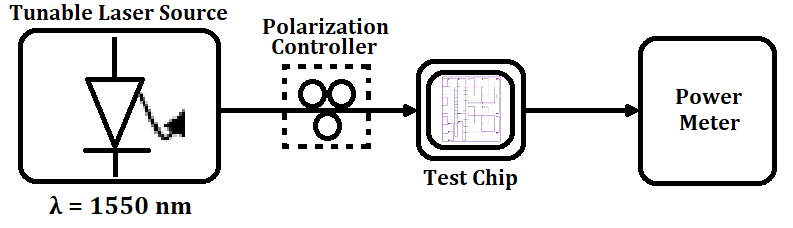
\includegraphics[width=8cm]{circuitdiag.png}
    \caption{Circuit used to perform loss/crossing measurements.}
    \label{fig:circuitdiag}
\end{figure}

A similar experiment performed by Bock \textit{et.al.} demonstrated a loss per crossing of -0.070 dB/crossing using a 50\% duty cycle and SWG pitch $\Lambda_f = 400$ nm \cite{BockPaper}. The experiment detailed in \cite{BockPaper} implements structures having 0, 1, 5, 10, 20, 40, and 80 crossings, with each structure having identical waveguide lengths to eliminate the effect of wire propagation loss. In contrast, we implement structures having 1, 5, and 11 crossings, with waveguide lengths as specified in table \ref{table:componentspecs} and shown in figure \ref{fig:klayout} of the appendix.
 
\begin{table}[!h]
\begin{tabular}{cccl}
\hline
\multicolumn{4}{c}{Fabricated Chip Specifications and Results} \\ \hline \hline
\multicolumn{1}{c|}{} & \multicolumn{1}{c|}{\begin{tabular}[c]{@{}c@{}}Strip Waveguide\\ Length ($\mu$m)\end{tabular}} & \multicolumn{1}{c|}{\begin{tabular}[c]{@{}c@{}}Uniform SWG\\ Length ($\mu$m)\end{tabular}} & \multicolumn{1}{c}{\begin{tabular}[c]{@{}c@{}}Measured \\ Loss (dB)\end{tabular}} \\ \hline
\multicolumn{1}{c|}{1 Crossing} & \multicolumn{1}{c|}{$210$} & \multicolumn{1}{c|}{$100$} & $-21.2(2)$ \\ \hline
\multicolumn{1}{c|}{5 Crossings} & \multicolumn{1}{c|}{$665$} & \multicolumn{1}{c|}{$300$} & $-22.1(2)$ \\ \hline
\multicolumn{1}{c|}{11 Crossings} & \multicolumn{1}{c|}{$1160$} & \multicolumn{1}{c|}{$610$} & $-24.1(7)$ \\ \hline
\end{tabular}
\caption{Length specifications and corresponding measured losses for fabricated chip components.}
\label{table:componentspecs}
\end{table}

\vspace{-2em}
\begin{figure}[!h]
    \centering 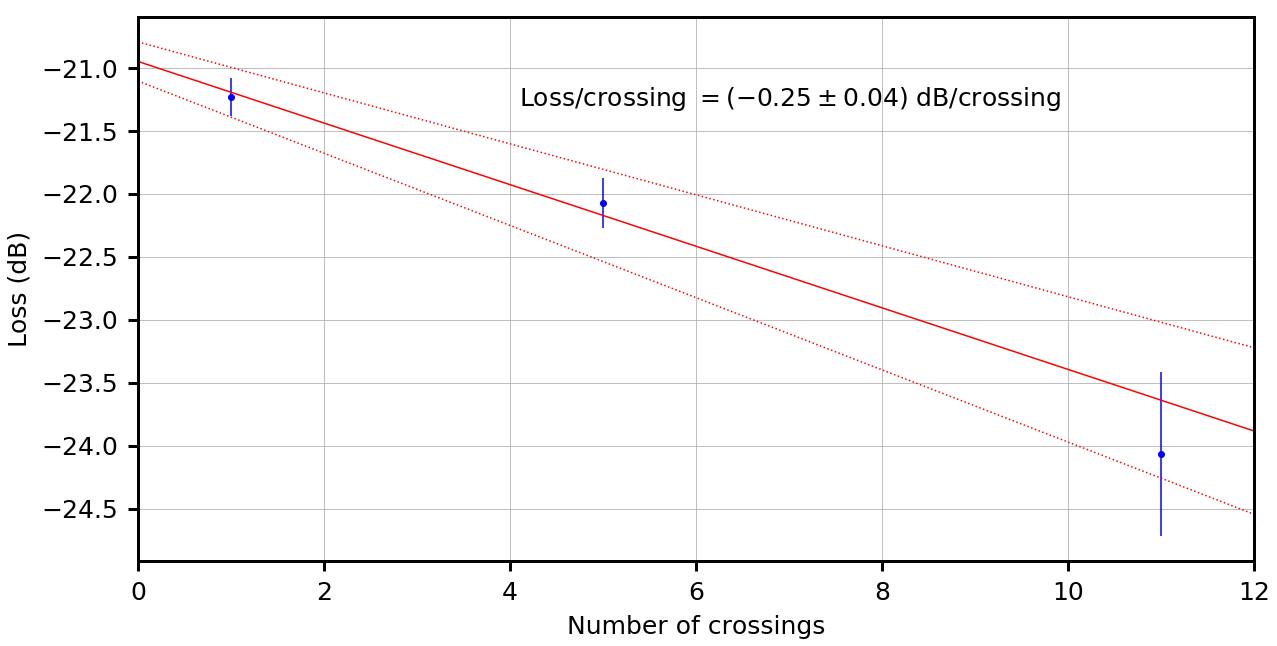
\includegraphics[width=8cm]{results.png}
    \caption{Measured losses for each fabricated crossing.}
    \label{fig:results}
\end{figure}
Loss per crossing is calculated as the slope of the error-weighted linear fit of measured losses, as shown in figure \ref{fig:results}. We obtain a result of $-(0.25 \pm 0.04)$ dB/crossing, which is significantly more loss than expected. However, this result comes from a small sample size, and is subject to several sources of error. For instance, loss measurements are highly sensitive to coupling efficiency between the input fibre and test chip. The manual fibre-chip coupling process introduces measurement errors that are difficult to minimize. 

The most notable sources of error arise from our crossing structures having differing waveguide lengths. For instance, longer structures are more likely to contain fabrication defects. Such defects would contribute to the measured loss in a way that steepens the linear fit, resulting in a larger loss per crossing value. Most notably, longer structures are subject to more wire propagation loss than shorter structures. Non-negligible propagation losses would also result in a steeper linear fit, corresponding to more loss per crossing. These effects can be drastically reduced in future SWG waveguide experiments by making all structures have similar dimensions. If these effects could be eliminated, we would expect a measured loss per crossing closer to the value demonstrated in \cite{BockPaper}.

\section{IV. Conclusion}
\vspace{-.1cm}
We have reported on the operation of subwavelength grating waveguide crossings, including simulation results and experimental measurements. Although our experimental measurements are not as expected, they have highlighted an important consideration in the design and testing of SWG waveguide devices. In particular, our experiment demonstrates the importance of regulating waveguide lengths to eliminate the effect of unwanted losses when testing such devices.

The low crosstalk and high output transmission values exhibited by SWG waveguide crossings make them strong candidates for the design of complex planar waveguide circuits. Notably, SWG waveguide crossings have the potential to facilitate the massive interconnectivity required for programmable logic. Combined with active photonic devices, meshes of SWG waveguide crossings form a potential architecture for optical logic platforms. Future experiments might build on the idea of using these meshes as a potential architecture for programmable logic gates.

\vspace{-1em}
\subsection{Acknowledgements}
\vspace{-1em}
\noindent The authors thank Hao Sun and Mostafa Khalil for assisting with chip design and testing. 
\bibliographystyle{IEEEtran}
\bibliography{mybib}

\pagebreak 

\onecolumngrid
\appendix
\section{Appendix}
\begin{figure}[!h]
    \centering 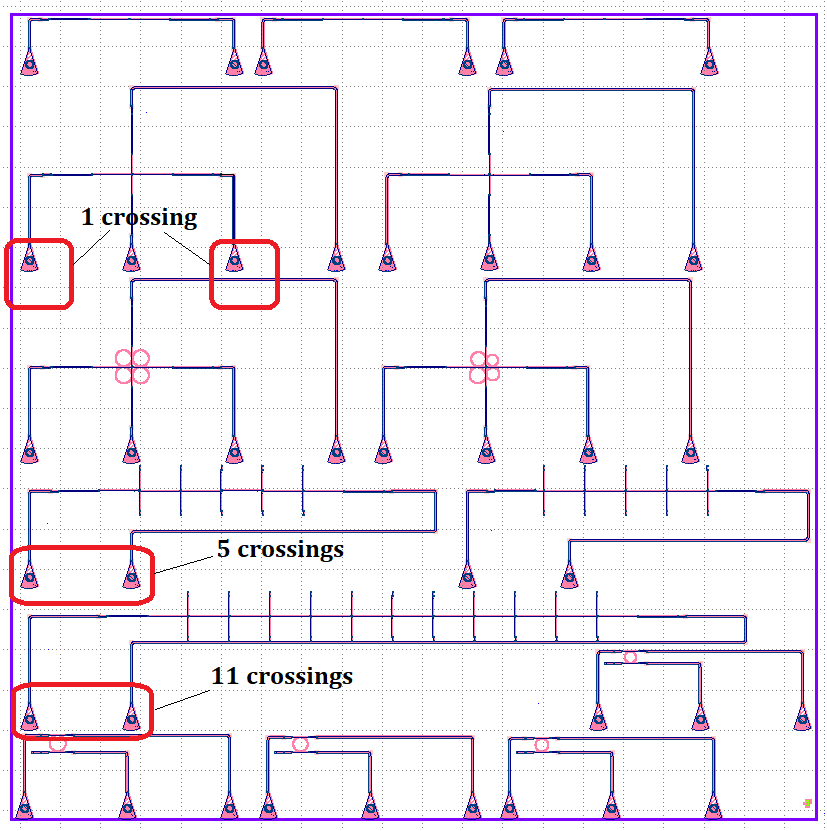
\includegraphics[width=11cm]{klayout.png}
    \caption{Layout of fabricated 1 mm$^2$ test chip. Input/output ports used in this experiment are highlighted with red boxes. The background grid consists of $50 \times 50 \text{ } \mu\text{m}^2$ squares.}
    \label{fig:klayout}
\end{figure}

\begin{figure}[!h]
    \centering 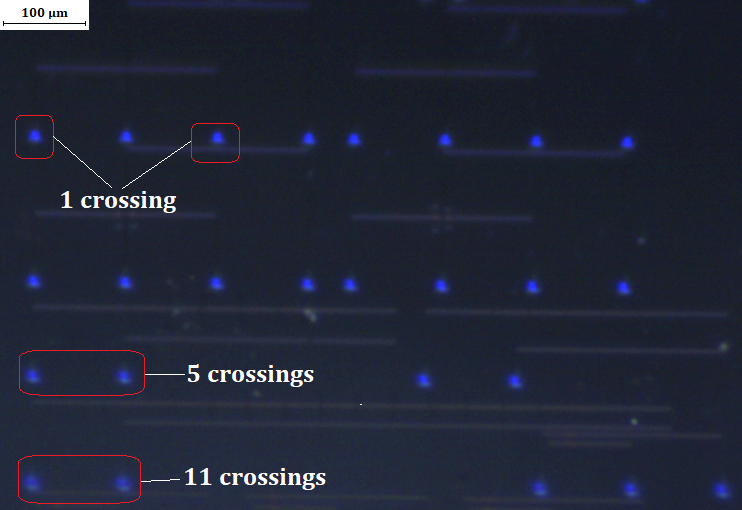
\includegraphics[width=10cm]{swgcrosschip.png}
    \caption{Microscope image of fabricated test chip. Input/output ports used in this experiment are highlighted with red boxes.}
    \label{fig:microscopelayout}
\end{figure}
\pagebreak 


\begin{figure}[htbp]
    \centering
    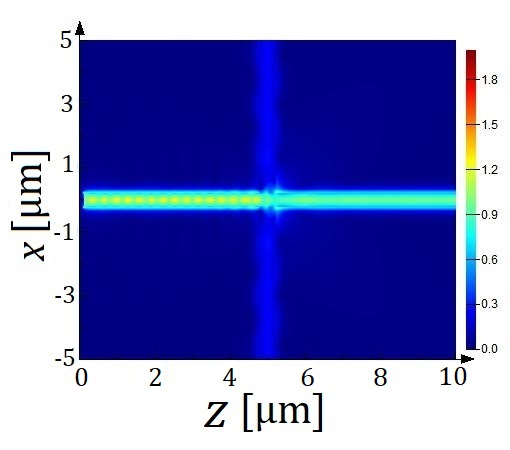
\includegraphics[width=8cm]{Regular_crossing.jpg}
    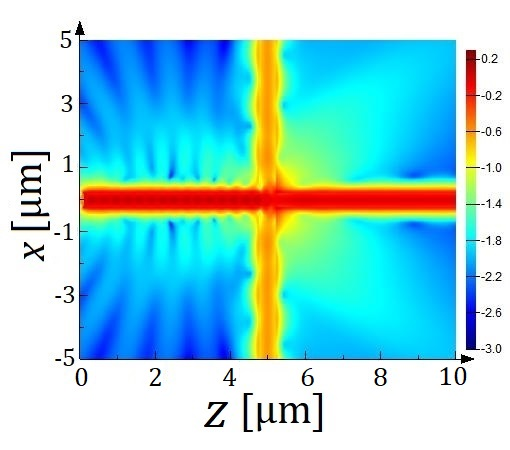
\includegraphics[width=8cm]{Regular_crossing_log.jpg}
    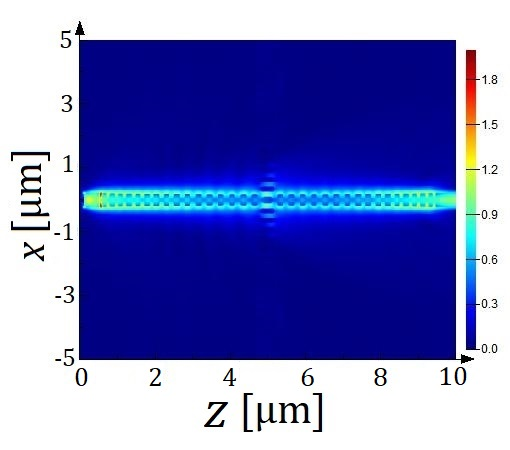
\includegraphics[width=8cm]{swg_bock_1.jpg}
    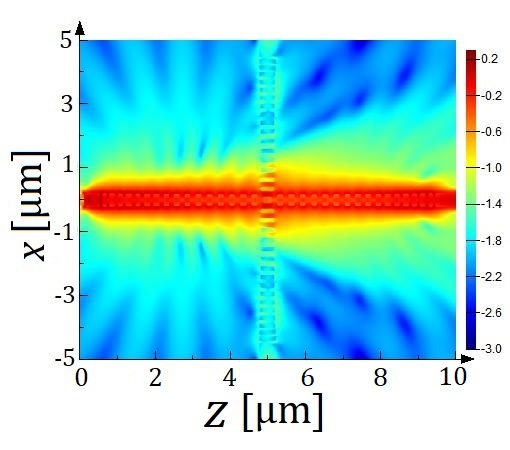
\includegraphics[width=8cm]{swg_bock_1_log.jpg}
    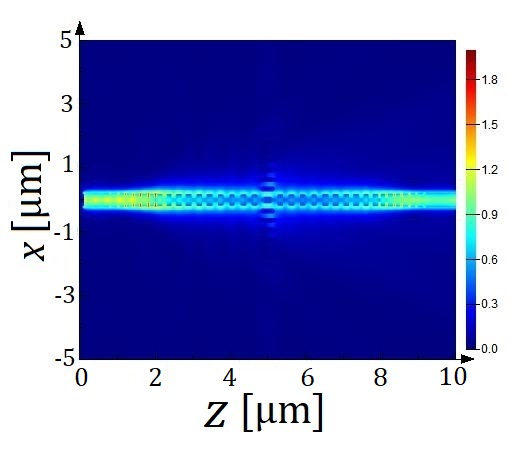
\includegraphics[width=8cm]{swg_bock_2.jpg}
    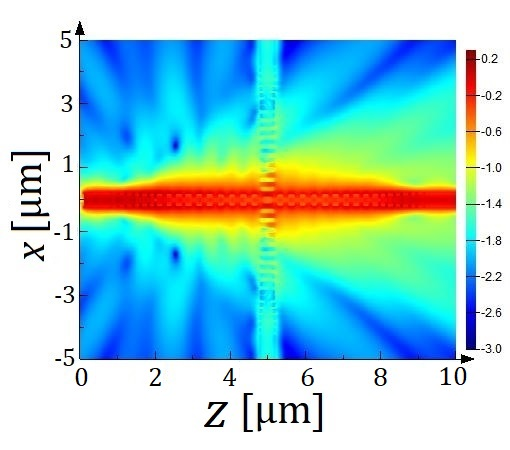
\includegraphics[width=8cm]{swg_bock_2_log.jpg}
    
    \caption{Simulated $E$-field magnitudes with $\lambda = 1550$ nm and input amplitude $=1$. Linear scale (left) and $\log_{10}$ scale (right). \\ \textbf{Top row}: Conventional strip waveguide crossing. Absence of lateral confinement at the intersection of the crossing results in scattering and high crosstalk. \\
    \textbf{Middle row}: SWG waveguide crossing with a linearly chirped and tapered transition region (design of figure \ref{fig:Bock}, top). \\
    \textbf{Bottom row}: SWG waveguide crossing with bridged and tapered transition region (design of figure \ref{fig:Bock}, bottom). }
    \label{fig:LumericalResults}
\end{figure}

\pagebreak

\begin{figure}[htbp]
    \centering
    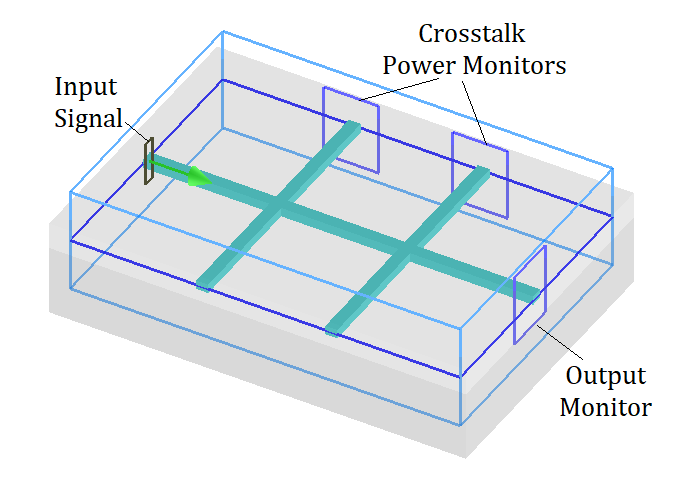
\includegraphics[width=8cm]{reg2diag.png}
    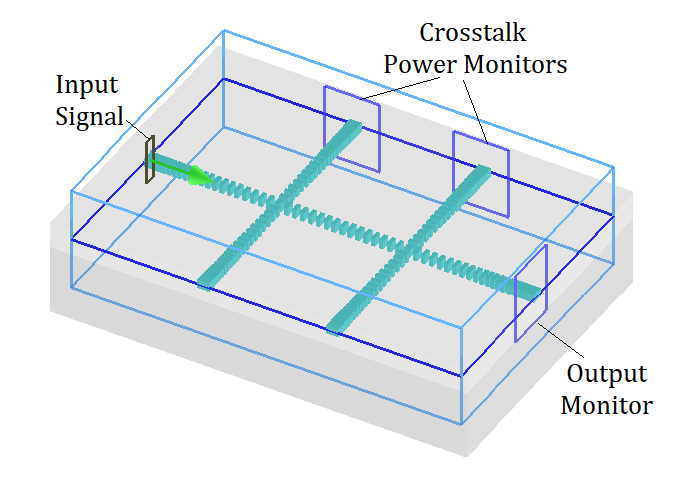
\includegraphics[width=8cm]{swg2diag.png}
    \caption{Layout of simulated double crossings discussed in section II. \\ \textbf{Left}: Double conventional strip waveguide crossing. \\ \textbf{Right}: Double SWG waveguide crossing with bridged taper transition regions.}
    \label{fig:diagsDouble}
\end{figure}

\begin{figure}[htbp]
    \centering
    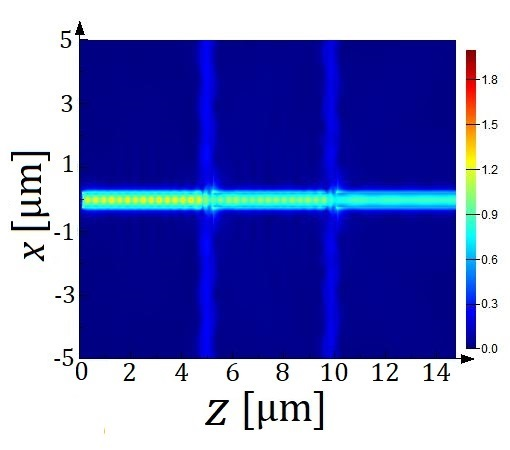
\includegraphics[width=8cm]{reg2cross.jpg}
    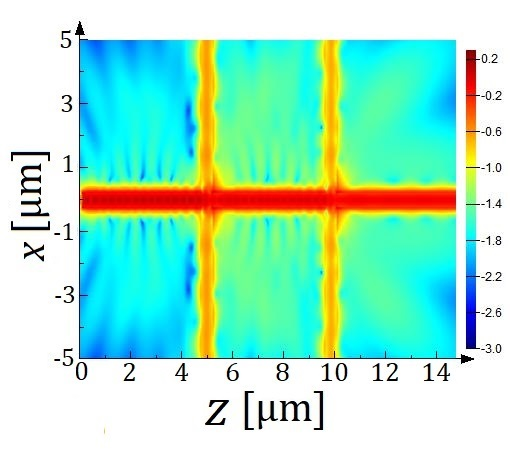
\includegraphics[width=8cm]{reg2cross_log.jpg}
    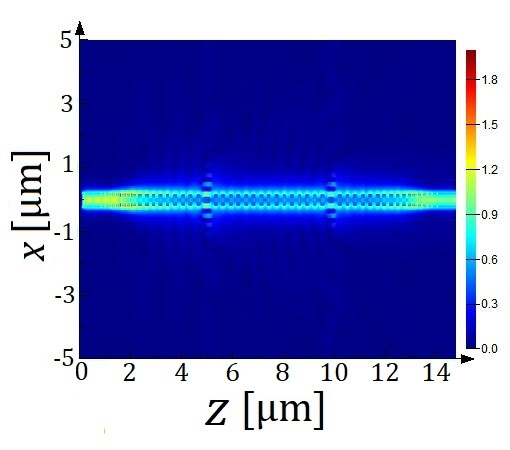
\includegraphics[width=8cm]{bridged2cross.jpg}
    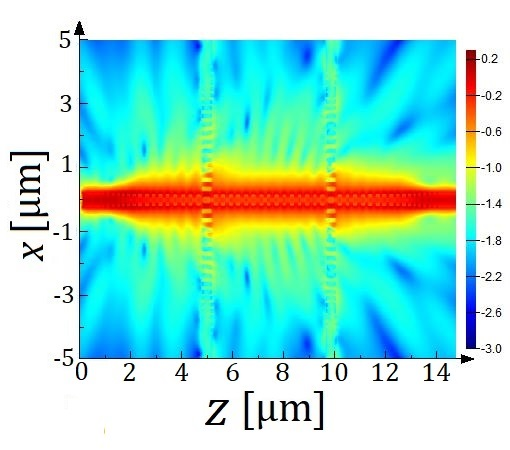
\includegraphics[width=8cm]{bridged2cross_log.jpg}
    
    \caption{Simulated $E$-field magnitudes with $\lambda = 1550$ nm and input amplitude $=1$. Linear scale (left) and $\log_{10}$ scale (right). \\ \textbf{Top row}: Field profile of two conventional strip waveguide crossings. \\
    \textbf{Bottom row}: Field profile of two SWG waveguide crossings connected by a uniform 50\% duty cycle SWG waveguide region. The transition region is bridged and tapered (design of figure \ref{fig:Bock}, bottom). }
    \label{fig:LumericalResultsDouble}
\end{figure}


\end{document}
